\chapter{Suggested solution}
\label{chp:suggested-solution}

In this chapter we'll present our solution to the problem.

\section{Modelling}



\subsection{Alternative model}

One alternative way to model the problem, is to skip the node splitting step of the previous model, and instead connect nodes directly, but stay below bandwidth by adding constraints for the total sum going out from each node. Which model to choose is -- as in every engineering matter -- a question of priorities. The first model is a bit harder to comprehend initially, but results in fewer total edges than the latter model does when n>3, as can be seen in \autoref{fig:models-compared}. Edge counts do not matter that much when n is low as finding a solution will occur in trivial time anyway, but the difference might be substantial when n is larger. \todo{If performance ends up being an issue for larger graphs, add a note here about more research being needed into optimizing performance, as alternative models might be an avenue to explore for achieving that.}

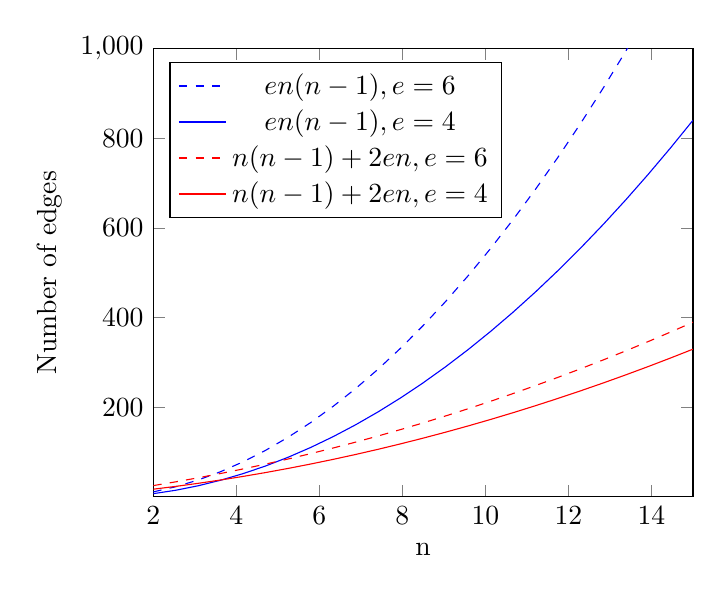
\begin{tikzpicture}
    \begin{axis}[
        xlabel={n},
        ylabel={Number of edges},
        xlabel near ticks,
        ylabel near ticks,
        legend pos=north west,
        xmin=2,
        ymin=1,
        ymax=1000,
        xmax=15]

    \addplot+[dashed, domain=2:15, mark=none, color=blue]{6*x*(x-1)};
    \addlegendentry{$en(n-1), e=6$}

    \addplot+[domain=2:15, mark=none, color=blue]{4*x*(x-1)};
    \addlegendentry{$en(n-1), e=4$}

    \addplot+[dashed, domain=2:15, mark=none, color=red]{x*(x-1) + 2*x*6};
    \addlegendentry{$n(n-1) + 2en, e=6$ }

    \addplot+[domain=2:15, mark=none, color=red]{x*(x-1) + 2*x*4};
    \addlegendentry{$n(n-1) + 2en, e=4$ }
    \label{fig:utility-latency}
    \end{axis}
%%    \caption{How the number of edges in the graph scales for different modeling techniques.}
\end{tikzpicture}


\section{The Algorithm}

Given the model, how do you efficiently find the "best" topology?

\section{Tuning}

How can the algorithm be tuned, and how was the parameters chosen?
